\makeatletter
\def\input@path{{headers/}}
\makeatother
\documentclass{beamer}

\usepackage{beamer_tom}
\usepackage{hyperref}

\usepackage{pythonhighlight}
\graphicspath{{./images/}{../../sharedimages/}}


\institute{INRIA Saclay}
\author{Thomas Moreau}
\title{
    Benchopt 1.8:\\
    Release highlights
}

\date{
    May 29, 2018
}

\setbeamertemplate{title page}[frame]
\collaborators[none]{\vskip-2em}
\def\extraLogo{\includegraphics[height=2.5cm]{logo_benchopt}}


\begin{document}

    \begin{frame}
        \titlepage
    %	\biblio{}
    \end{frame}

    \frame{
        \frametitle{Improved support for general ML workflows}

        Benchopt 1.8 improves the support for benchmarking full ML workflows,\\[.5em]
        {\centering
            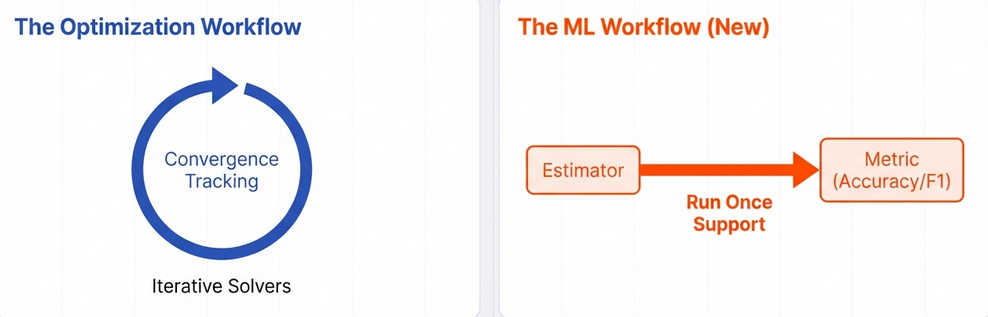
\includegraphics[width=\textwidth]{ml_workflows.png}\\[2em]
        }

        \begin{columns}
            \column{.58\textwidth}
            Easy configuration:\\[.5em]
            \inputpython{benchopt_objective.py}{4}{7}
            \column{.38\textwidth}

            \myitem{} Easier tests\\
            \myitem{} Improved doc\\
            \myitem{} ...\\

        \end{columns}



    }

    \frame{
        \frametitle{Visualization and reporting improvements}

        Big work by @Etyl (aka Hippolyte) on a customization API for the plots.\\[1em]

        \begin{columns}
            \column{.53\textwidth}
            \inputpython{custom_plot.py}{1}{12}
            \column{.43\textwidth}
            \myitem{} Can create tables\\[.5em]
            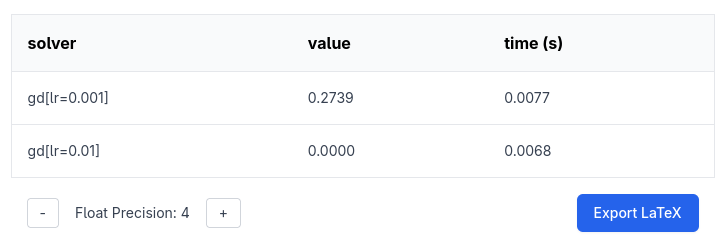
\includegraphics[width=\textwidth]{benchopt_table.png}\\[.3em]

            \myitem{} Improve display on mobile\\[1em]
            \myitem{} + various fixes...\\
        \end{columns}
    }
    {
    \usebackgroundtemplate{%
    \begin{picture}(400, 300)(0, -30)
    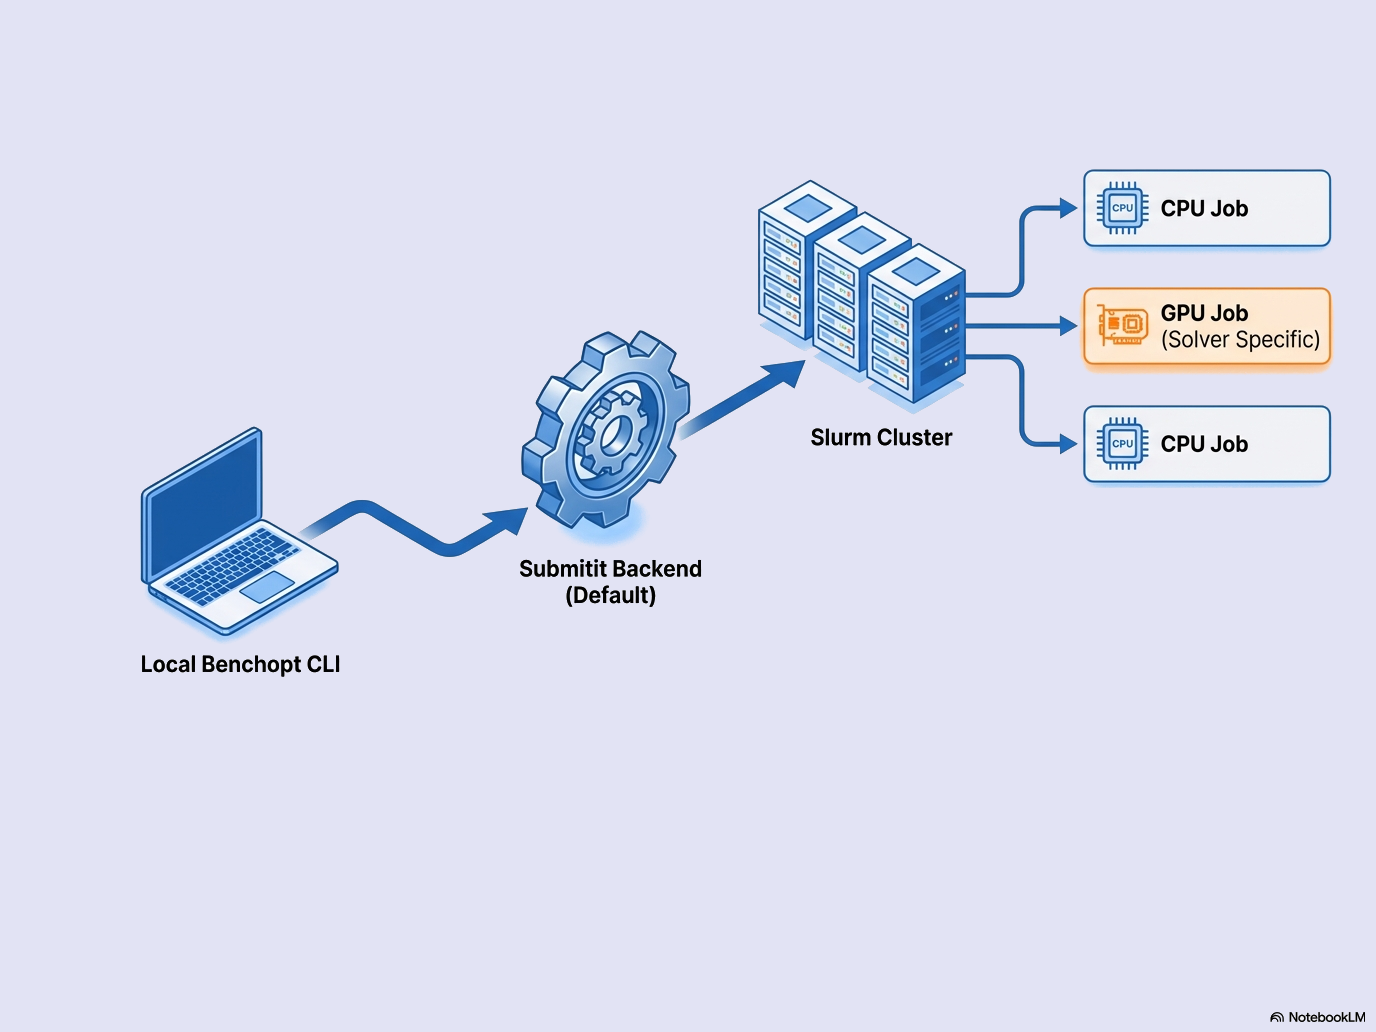
\includegraphics[
        width=1\paperwidth
    ]{parallel_backend}%
    \end{picture}
}
    \frame[t]{
        \frametitle{Scaling with Advanced Parallel Backends}

        \begin{columns}[T]
            \column{.4\textwidth}
            \begin{itemize}
                \item  Default backend uses \texttt{submitit}\\[.5em]
                \item Allow for solver specific control over resources\\[.5em]
            \end{itemize}
            \column{.6\textwidth}
            \vskip11em
            \inputpython{solver_config.py}{1}{10}
        \end{columns}





    }
    }



    \frame{

        {\centering \huge Get started with Benchopt 1.8\\[2em]}

        \highlightbox{
            \centering pip install -U benchopt
        }
        \vskip2em

        \begin{columns}
            \column{.43\textwidth}
            \textcolor{C0}{\bf Documentation}\\[.5em]
            \myitem{} Improved ML workflow\\
            \myitem{} Custom plot guide\\
            \myitem{} \parbox[t]{.8\textwidth}{Gallery of examples\\\emph{minimal, nanoGPT}}\\

            \column{.30\textwidth}
            \textcolor{C0}{\bf Join Us}\\[.5em]
            \myitem{} Discord server\\
            \myitem{} Github Repo\\

            \column{.22\textwidth}
            \centering
            
\includegraphics[width=\textwidth]{qr-code_discord.png}\\
        \end{columns}

        \strongpoint{Please consider starring the repo to help gain visibility!}
    }

\end{document}